 \documentclass{sciposter}
\usepackage{lipsum}
\usepackage{epsfig}
\usepackage{amsmath}
\usepackage{amssymb}

% Para Tablas
\usepackage{multicol}
\usepackage{multirow}

% Para gráficas propias
\usepackage{pst-all}
\usepackage{multido,pstricks}

\usepackage{graphicx,url}

% Idioma
\usepackage[spanish]{babel}   

% Codificación
\usepackage[utf8]{inputenc}
%\usepackage{fancybullets}

% Se pueden crear comandos propios de theorems
\newtheorem{Def}{Definici\'on}


% Título del proyecto
\title{Proyecto Final\\ Recomendador de Pel\'iculas}

% Nombre de los autores
\author{Pedro Flores, Miguel Figueira, David Padrino}

% Dirección de la Universidad
\institute 
{Escuela de Computación\\
Facultad de Ciencias \\ 
Universidad Central de Venezuela (UCV)\\
  Av. Paseo Los Ilustres, Los Chaguaramos, Caracas, Venezuela}
  
% Correo electrónico


% Logos de universidad y facultad

\rightlogo[1]{logociens}
\leftlogo[1.2]{logo-ucv}

\begin{document}
%define conference poster is presented at (appears as footer)

\conference{{\bf II-2015}, Papers sobre Miner\'ia de Datos, Mayo de 2016, Caracas, Venezuela}

%\LEFTSIDEfootlogo  
% Uncomment to put footer logo on left side, and 
% conference name on right side of footer

% Some examples of caption control (remove % to check result)

%\renewcommand{\algorithmname}{Algoritme} % for Dutch

%\renewcommand{\mastercapstartstyle}[1]{\textit{\textbf{#1}}}
%\renewcommand{\algcapstartstyle}[1]{\textsc{\textbf{#1}}}
%\renewcommand{\algcapbodystyle}{\bfseries}
%\renewcommand{\thealgorithm}{\Roman{algorithm}}

\maketitle

%%% Begin of Multicols-Enviroment
\begin{multicols}{3}

%%% Abstract
\begin{abstract}
% BEGIN MINERIA UCV
En este art\'iculo se dan a conocer los conceptos b\'asicos requeridos para empezar a comprender los sistemas de recomendaci\'on, espec\'ificamente bajo el uso de filtrado colaborativo.\\
La plataforma Kaggle permite utilizar datasets para la resoluci\'on de determinados problemas de miner\'ia de datos. El problema en cuesti\'on es la realizaci\'on de un sistema que sirva de recomendador de pel\'iculas de acuerdo a ciertas votaciones realizadas por un grupo de usuarios a un grupo de pel\'iculas de diferentes g\'eneros, duraciones y clasificaciones.\\
Al trabajar con una cantidad tan grande de elementos hubo problemas al momento de realizar an\'alisis  porque el proceso se hacia un tanto tedioso y la lenta respuesta de los computadores hizo que las pruebas fueran la parte del proyecto que m\'as tiempo demandara..\\
Los resultados de las predicciones fueron acertados hasta cierto punto, debido a que la cantidad de votaciones, a pesar de ser en gran n\'umero, no fue suficiente para realizar una predicci\'on m\'as acertada y precisa. Sin embargo se lograron predecir todos los valores para los usuarios en cuesti\'on, m\'as adelante se hablar\'a al respecto con mayor detenimiento

% END MINERIA UCV
\end{abstract}

%%% Introduction
\section{Introducci\'on}
\PARstart{E}{l} grupo de desarrollo GroupLens busca desarrollar un recomendador de pel\'iculas basado en filtrado colaborativo llamado \emph{Movielens}, el cual se espera que funcione de acuerdo a  1,000,209 valoraciones o ratings de 6040 usuarios de MovieLens hacia 3900 pel\'iculas. Este conjunto de datos es del a\'no 2000 aproximadamente.
\\
Para la realizaci\'on de este proyecto fue desarrollada una aplicaci\'on en la herramienta \emph{RShiny}, que permite interactuar con el algoritmo, hacer selecciones de datos y as\'i de esta manera mostrar los resultados de forma estructurada y en una sola ventana. La mencionada herramienta fue utilizada para algunos gr\'aficos que se muestran en el presente art\'iculo.
\section{An\'alisis Exploratorio de Datos}
Se proveen tres archivos en base a los cuales se tomar\'an los datos (users.dat, ratings\_for\_kaggle\_comp.csv y movies.dat) y un archivo en base al que se realizar\'an las lecturas (sample\_submission.csv) en donde se puede observar cu\'al usuario valor\'o a cu\'al pel\'icula.\\
Se realiz\'o una lectura de los archivos y para poder utilizarlos dentro del procesamiento fue necesario cambiar su formato.\\
En la siguiente estructura se muestra la data cruda, luego de cambiado su formato quedo estructurado en columnas "limpias".
\begin{itemize}
\item users.dat: Esta en un rango entre 1 y 6040\\
El formato de las columnas es el siguiente:\\
\begin{center}
\emph{UserID::Gender::Age::Occupation::Zip-code}
\end{center}
Toda la informaci\'on demogr\'afica fue dada voluntariamente por los usuarios, los cuales fueron los \'unicos que fueron agregados al conjunto.\\
El g\'enero es denotaro por "M" para hombres y "F" para mujeres.\\
Las edades fueron seleccionadas de acuerdo a los siguiente rangos:
\begin{center}
	*  1:  "menor de 18"\\
	* 18:  "18-24"\\
	* 25:  "25-34"\\
	* 35:  "35-44"\\
	* 45:  "45-49"\\
	* 50:  "50-55"\\
	* 56:  "56+"\\
\end{center}

La ocupaci\'on es elegida de acuerdo a los siguientes elementos:
\begin{center}
	*  0:  "other" or not specified\\
	*  1:  "academic/educator"\\
	*  2:  "artist"\\
	*  3:  "clerical/admin"\\
	*  4:  "college/grad student"\\
	*  5:  "customer service"\\
	*  6:  "doctor/health care"\\
	*  7:  "executive/managerial"\\
	*  8:  "farmer"\\
	*  9:  "homemaker"\\
	* 10:  "K-12 student"\\
	* 11:  "lawyer"\\
	* 12:  "programmer"\\
	* 13:  "retired"\\
	* 14:  "sales/marketing"\\
	* 15:  "scientist"\\
	* 16:  "self-employed"\\
	* 17:  "technician/engineer"\\
	* 18:  "tradesman/craftsman"\\
	* 19:  "unemployed"\\
	* 20:  "writer"\\
\end{center}
\item ratings\_for\_kaggle\_comp.csv: \\
Todos los elementos contenidos en este archivo siguen el siguiente formato:\\
\begin{center}
\emph{UserID::MovieID::Rating::ID}
\end{center}
- UserIDs: Rango entre 1 y 6040.\\
- MovieIDs: Rango entre 1 y 3952.\\
- Ratings: son hechos en base a 5 estrellas .\\
- ID: Una mezcla de los UserIDs con MovieIDs separados por \emph{underscore (\_)}.\\
\item movies.dat: La informaci\'on dentro de este archivo est\'a de la siguiente forma:\\
\begin{center}
\emph{MovieID::Title::Genres}
\end{center}
Los t\'itulos son id\'enticos a los provistos por IMDB, incluyendo a\'no de lanzamiento.\\
Los g\'eneros estan separados por \emph{pipe} y se toman de la siguiente lista:
\begin{center}
	* Action\\
	* Adventure\\
	* Animation\\
	* Children's\\
	* Comedy\\
	* Crime\\
	* Documentary\\
	* Drama\\
	* Fantasy\\
	* Film-Noir\\
	* Horror\\
	* Musical\\
	* Mystery\\
	* Romance\\
	* Sci-Fi\\
	* Thriller\\
	* War\\
	* Western\\
\end{center} 

\item sample\_submission.csv: Como se explic\'o anteriormente es el dataset central con el cual se va a realizar el trabajo, permite ver cu\'ales usuarios han realizado valoraciones a cu\'ales pel\'iculas. \\
Se muestra en el siguiente formato:\\
\begin{center}
\emph{UserID::Rating::ID}
\end{center}
ID: Representa un h\'ibrido de la forma UserID\_MovieID.\\
El resto de los elementos son intuitivos de entender.\\\\\\\\
\end{itemize}

Adem\'as de los cambios de formato a los archivos, se realiz\'o el borrado de aquellos usuarios que no hayan votado a ninguna pel\'icula y  aquellas pel\'iculas que no fueron votadas, de manera que no afectara el resultado del procesamiento.


\begin{figure}
\begin{center}
 	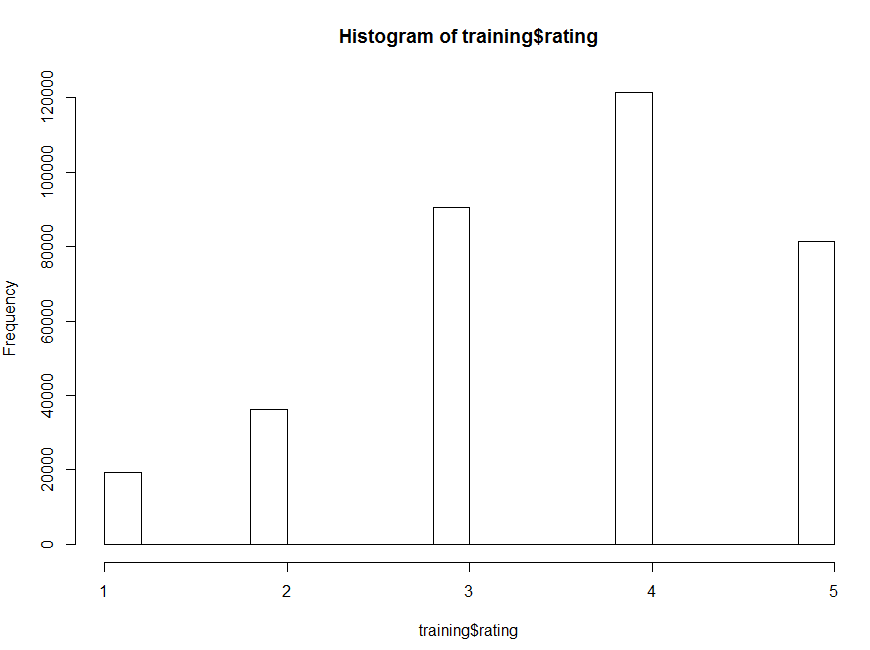
\includegraphics[scale=0.75]{votos_por_rating}
\end{center}
\caption{ distribuci\'on de las rating de las pel\'iculas }\label{fig:votosrating}
\end{figure}


\begin{figure}
\begin{center}
 	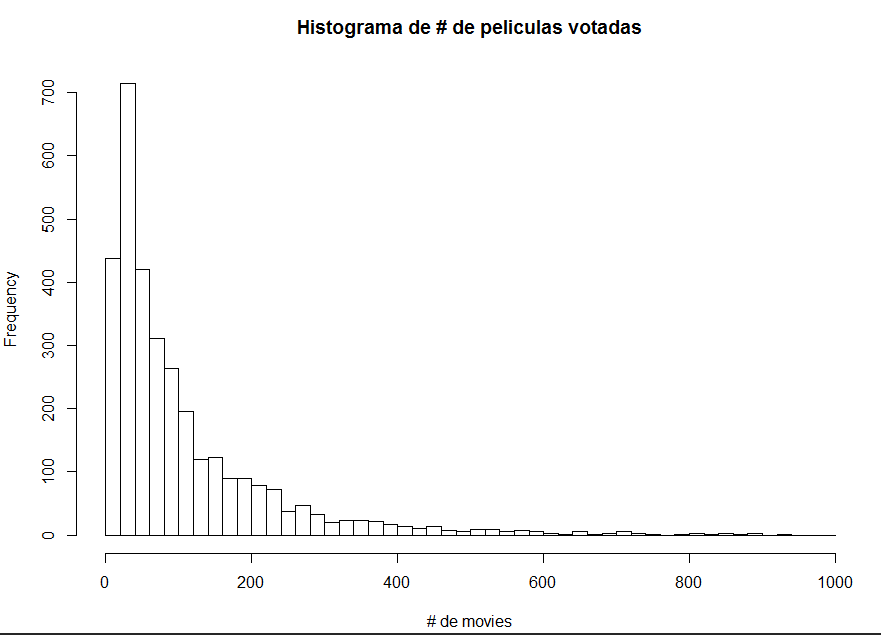
\includegraphics[scale=1]{histograma_votos}
\end{center}
\caption{distribuci\'on por n\'umero de pel\'iculas votadas por usuario , la mayor\'ia de los usuarios vot\'o entre 20 y 40 pel\'iculas  }\label{fig:distribvotos}
\end{figure}





% Esta sección va a depender de los proyectos, podría llamarse simplemente PReprocesamiento
\section{Preprocesamiento|Crear Matriz Dispersa}

% Usando subsecciones
%  Creo que tal vez aquí deberíamos mostrar el histograma para ejemplificar que algunos usuarios tienen poca data.. pero ni idea xD

\subsection{Crear data de entrenamiento y prueba}
Ya que la data que provee Kaggle solo ofrece data de entrenamiento, se procede a crear una data personalizada de entrenamiento y otra de prueba a partir de esa data inicial.\\ 
Para ello se usa una t\'ecnica de muestreo estratificado tomando el 70\% de las votaciones realizadas por los usuario como entrenamiento y el 30\%  restante como prueba, ya que si se toma el 70\% es posible que alg\'un usuario no tenga ninguna pel\'icula dentro de la data de entrenamiento.


% posiblemente sería bueno hacer la referencia a la librería reshape en donde menciono la función acast , no lo hago xq no se como hacerlo y me da ladilla buscarlo ahorita xD
\subsection{Crear matriz dispersa}
Viendo el formato de la data en la figura N, es necesario transformarla para  tener una matriz dispersa donde los usuarios sean las instancias (o filas), las pel\'iculas sean las columnas y los elementos de la matriz son los ratings o valoraciones de los usuarios. Para lograr esto se hace uso de la funci\'on \emph{acast} de la biblioteca \emph{reshape}.\\ 
Es bueno mencionar que la funci\'on \emph{acast} retorna elementos de clase \emph{vector}, \emph{matrix}, o \emph{array}


% Breve definición del algoritmo escogido por ustedes y razonamiento detrás de esto.
\section{Filtrado Colaborativo }
 
El algoritmo de filtrado colaborativo es ampliamente  conocido por usarse en sistemas de recomendaci\'on, en nuestro caso usamos el algoritmo basado en usuario-usuario y se basa en la premisa de que si un usuario A se parece a un usuario B en cu\'anto a las pel\'iculas que ha votado , entonces es posible que el usuario A tenga la misma valoraci\'on sobre otras pel\'iculas que ha evaluado el usuario B.
Adem\'as cabe destacar que para este usar este algoritmo solo usamos las valoraciones dejando de lado , la descripci\'on de usuario como edad y ocupaci\'on , o informaci\'on de las pel\'iculas como g\'enero o a\~no

Para lograr esto hicimos uso de una biblioteca en R llamada \emph{Recommenderlab} usandola de la siguiente manera: 

Luego de todo el preprocesamiento se procedi\'o a convertir la matriz de votaciones en un tipo especial de matriz heredado de la clase ‘Rating Matrix’ (espec\'ificamente \emph{RealRatingMatrix}), con la cual permite hacer el proceso de recomendaci\'on|predicci\'on de acuerdo a lo establecido en la biblioteca.\\

Una vez con la matrix de la clase \emph{RatingMAtrix} se inicia el proceso de recomendaci\'on , en el cual se utilizar\'a el comando \emph{Recommender} basado en usuario (UBCF), con una lista de par\'ametros adicionales como: ‘Z-Score’ , que es el m\'etodo de normalizaci\'on, ‘Jaccard’ como medida de similaridad  (en algunas publicaciones es sugerida esta medida para estos casos de recomendaci\'on),  ‘nn’ representa el n\'umero de usuarios en base a los que se realizar\'an las recomendaciones  y por \'ultimo minRating, que representa el menor valor a partir del cual se realizar\'an las predicciones.


\begin{figure}
\begin{center}

 	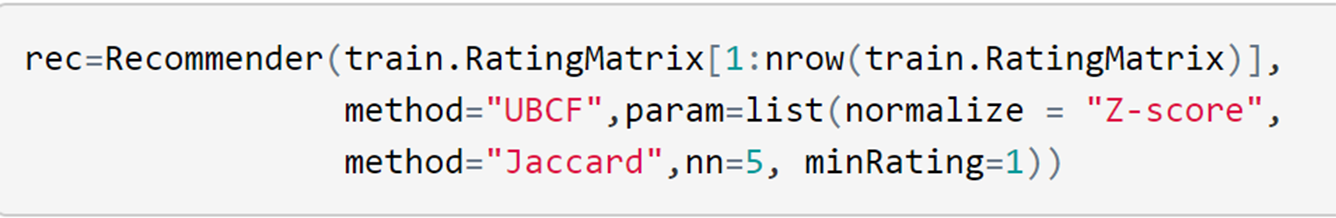
\includegraphics[scale=0.65]{rec6}
\end{center}
% Leyenda de cualquier figura, sea tabla o no
\caption{ genera rec que es el modelo necesario para calcular posteriormente las predicciones }\label{fig:rec5} % identificador de la figura
\end{figure}



Para las predicciones se usar\'a el comando \emph{predict}, pasando como par\'ametros el modelo obtenido anteriormente, junto a la RatingMatrix creada anteriormente.

\begin{figure}
\begin{center}

 	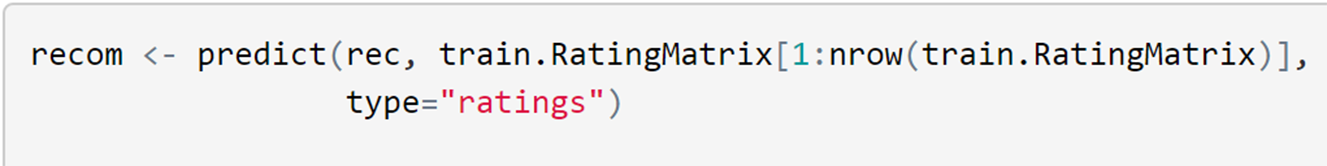
\includegraphics[scale=0.65]{recom4}
\end{center}
\caption{ c\'odigo para generar el modelo para luego generar las recomendaciones con predict }\label{fig:predict}
\end{figure}


Luego de ordenar y limpiar los datos se pueden apreciar los siguientes resultados: 

Predicciones de ratings que asignar\'a un usuario sobre un determinado n\'umero de pel\'iculas:

\begin{figure}
\begin{center}

 	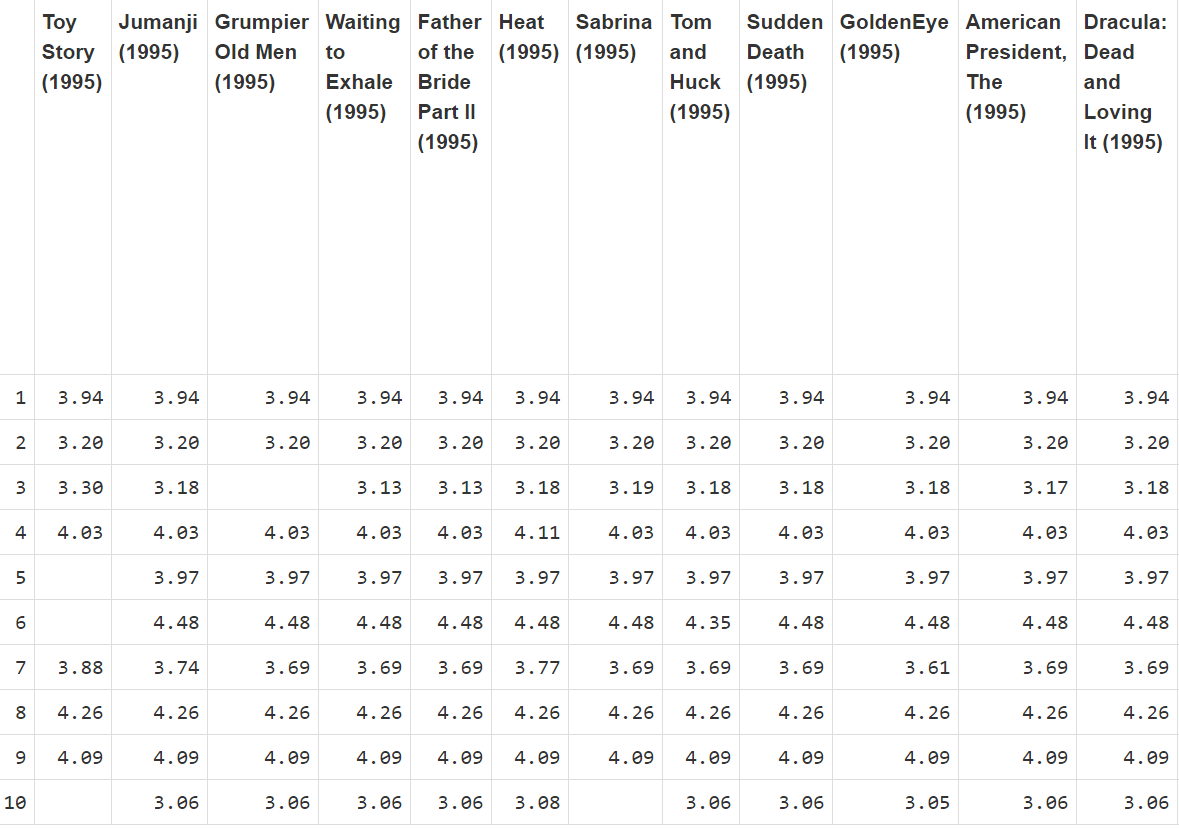
\includegraphics[scale=0.75]{predicciones}
\end{center}
\caption{ matriz resultado de las predicciones, los espacios en "blanco" es porque ya hab\'ian sido puntuados por el usuario}\label{fig:predicciones}
\end{figure}


\begin{figure}
\begin{center}

 	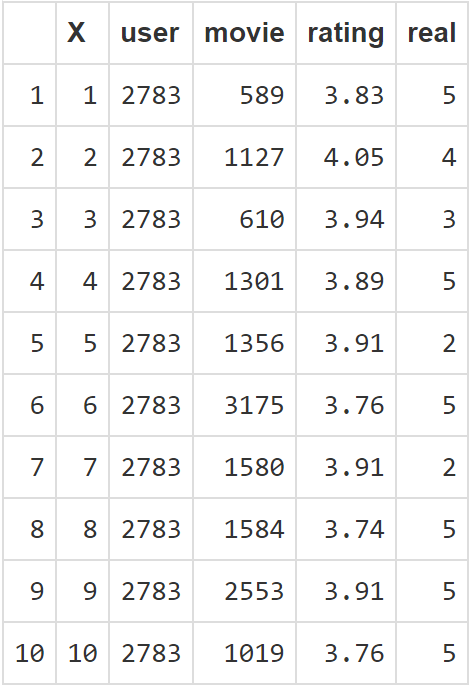
\includegraphics[scale=0.75]{comparacion}
\end{center}
\caption{ Comparaci\'on del resultado de las puntuaciones predichas con las puntuaciones reales: }\label{fig:comparacion}
\end{figure}



\begin{figure}
\begin{center}

 	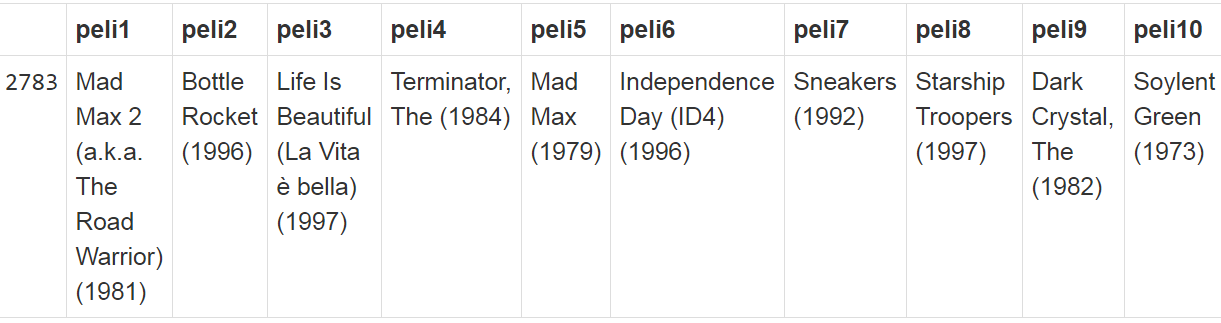
\includegraphics[scale=0.75]{recomendar}
\end{center}
\caption{ Lista de 10 pel\'iculas recomendadas a un usuario espec\'ifico: }\label{fig:recomendar}
\end{figure}


\section{Evaluaci\'on de Modelo}

\begin{figure}
\begin{center}
 	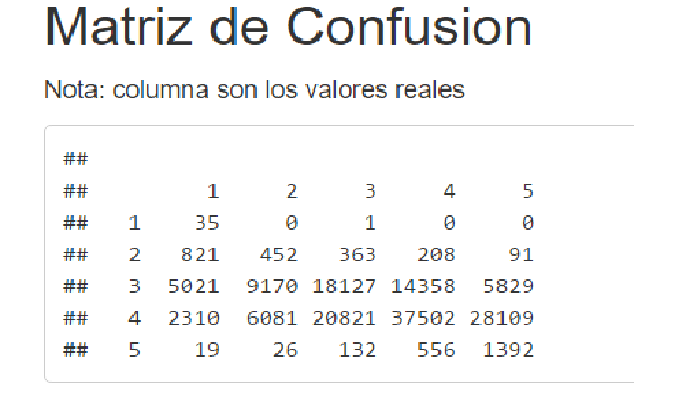
\includegraphics[scale=1]{MC}
\end{center}
\caption{ Comparaci\'on del resultado de las puntuaciones predichas con las puntuaciones reales, las filas son el resultado del algoritmo }\label{fig:mc}
\end{figure}

\subsection{Observaciones de la Matriz de Confusi\'on}
\begin{itemize}
\item Casi todos los que predijo como 1 eran realmente 1
\item Los 4 y los 3 los predijo bastante bien, entendiendo que la diferencia entre un 4 y un 3 no es mucha.
\item Los que eran realmente 1 los predijo casi todos como 2,3 o 4
\end{itemize}


\section{Resultados | Conclusi\'on}

Los sistemas de recomendaci\'on son herramientas muy \'utiles al momento de mejorar la experiencia del usuario con una aplicaci\'on o sitio web debido a que brindan la sensaci\'on de que el sistema conociera los gustos del usuario e hiciera recomendaciones en base a ellos, evidentemente todo es una abstracci\'on de lo que realmente es.\\
Con el presente proyecto y sus resultados se pudo observar que es necesario tener un cluster para poder generar recomendaciones en tiempo real debido a la gran cantidad de datos y procesamiento que se necesitan para poder realizar predicciones y recomendaciones acertadas en un tiempo prudencial.\\

Analizando la figura \ref{fig:predicciones}  se puede observar que los resultados no son los mejores, es decir, repite muchos valores de recomendaci\'on para un mismo usuario, lo cual posiblemente es una consecuencia de no contar con suficientes datos, adem\'as de que muchos usuarios tienen muy pocas recomendaciones como se puede observar en la figura \ref{fig:distribvotos} donde pocos usuarios tienen m\'as de 60 pel\'iculas votadas ,e incluso una cantidad significativa de personas tiene menos de 20 pel\'iculas calificadas.

Adem\'as de que las valoraciones del rating '1' las predice bastante mal como se menciona en la secci\'on Evaluaci\'on de Modelos, debido a que existe una diferencia significativa entre la cantidad de pel\'iculas calificadas como 3,4,5 con pel\'iculas calificadas con 1, como se puede apreciar en la figura \ref{fig:votosrating}
\\
%%%FALTA
%%% References
%% Note: use of BibTeX als works!!
 
\bibliographystyle{plain}
\begin{thebibliography}{1}

\bibitem{Flusser:Suk:93}
Michael Hahsler
\newblock recommenderlab: A Framework for Developing and
Testing Recommendation Algorithms.
\newblock  2011.

\bibitem{Hu:62}
Linux Uncle.
\newblock Using R package, recommenderlab, for predicting ratings for MovieLens data.
\newblock 2014.
\newblock  https://ashokharnal.wordpress.com/2014/12/18/using-recommenderlab-for-predicting-ratings-for-movielens-data/


\bibitem{Meijster:Wilkinson:PAMI}
inside-R.org.
\newblock Similarity and Dissimilarity Functions,
\newblock http://www.inside-r.org/packages/cran/sets/docs/similarity


\bibitem{Meijster:Wilkinson:PAMI}
wikipedia.org,
\newblock Jaccard index,
\newblock  https://en.wikipedia.org/wiki/Jaccard




\end{thebibliography}

\end{multicols}

\end{document}









